\chapter{Collisional effects on reflectometry fluctuation spectra} \label{ch:Spec_vs_nu}
\graphicspath{{chapter6_ys/}}
\minitoc

In the previous chapter, we have observed various differences of the broadband contribution $E_\mathrm{BB}$ between the LOC and SOC regimes, and between ICRH and LH plasmas. In this chapter, we turn to a possible explanation of these observations, by investigating the dependence of $E_\mathrm{BB}$ on collisionality.

At low density, we observed that $E_\mathrm{BB}$ increases slowly with density. However, further increasing the density, $E_\mathrm{BB}$ becomes strongly dispersed at fixed density, making it difficult to identify a clear trend. On the other hand, since the density affects the plasma collisionality, which in turn is known to affect the growth rate of instabilities, we decided to investigate the dependence of $E_\mathrm{BB}$ on collisionality, as this might given an indication whether the type of dominating instability is related to the observations of $E_\mathrm{BB}$.

The link between dominating instability and reflectometry frequency spectra has been extensively studied in terms of the quasi-coherent (QC) components in the spectra \cite{Arnichand_2014_NF}. Specifically, the disappearance of the QC modes has been proved to be a marker of the stabilization of the TEM instability \cite{Arnichand_2015_Thesis, Zhong_2016_PoP, Lee_2018_PoP}. We here wish to verify the possibility that a transition in the dominant instability may affect also the other components of the frequency spectra, i.e. the broadband (BB) and low-frequency (LF) components. This could be a suitable explanation for the observed trends of $E_\mathrm{BB}$ with different confinement regimes and heating methods.

However, linking the frequency spectra to the dominating instability by calculating the growth rates at different collisionality for the whole database would be impossible from the computational point of view. Therefore, in this chapter, we focus on linking changes in the BB and LF components with changes in the collisionality, by studying the dependence of the spectral properties (energy, width, shape) of the BB and LF components on collisionality. Section \ref{sec:spec_OH} first investigates the dependence of the BB component on collisionality in Ohmic plasmas and then discusses the possible interpretation in terms of a transition of dominant instability. This is based on the results of earlier gyrokinetic simulations and is supported by additional analysis of the density peaking and the LF component. Then, the study is extended to L-mode plasmas with ICRH and LH heating and possible interpretations are given. Additional discussion and perspectives are provided in section \ref{discussion_perspective}.


\section{Dependence of frequency spectrum on collisionality in Ohmic plasmas} \label{sec:spec_OH}

%In previous work, the transition from the LOC to SOC confinement regime has been attributed to a change in dominant micro-instability from TEM to ITG modes \cite{Angioni_PoP_2005_LOCSOC_TEMITG,Erofeev_2017_NF}. Linear gyrokinetic simulations with GENE for an Ohmic discharge with an $I_p$ scan (Tore Supra \#48102) have confirmed that the TEM instability dominates at high $I_p$ (LOC), whereas ITG dominates at low $I_p$ (SOC) \cite{Arnichand_2014_NF,Hacquin_2016_PoP,Citrin_2017_PPCF}. Therefore, in order to get a deeper understanding of the different Ohmic confinement regimes,.

%In Ohmic plasmas, The transition from the LOC to SOC confinement regime has been attributed in previous studies to a change in the dominant instability from trapped electron modes (TEM) to ion temperature gradient (ITG) modes \cite{Angioni_PoP_2005_LOCSOC_TEMITG,Erofeev_2017_NF}. Experimentally, this connection between the confinement regimes and the dominant instabilities has also been studied through the dependence of the density peaking and intrinsic rotation on collisionality in various devices, such as Alcator C-Mod and ASDEX Upgrade \cite{Rice_2012_PoP,Lebschy_2018_NF}. In these studies, collisions have been found to have a crucial impact on the determination of the LOC-SOC transition, since collisions could affect the trapped particle modes via the detrapping mechanism, i.e. collisions tend to stabilize the TEM modes.

As mentioned in section \ref{sec:effect_collision}, the LOC regime and SOC regime in Ohmic plasmas have been connected with the microinstability of TEM and ITG, respectively, and collisions has a crucial impact on the determination of the LOC-SOC transition. Therefore, to understand the difference of $E_\mathrm{BB}$ in the LOC and SOC egimes, this section studies the dependence of the spectral characteristics on effective collisionality. The effective collisionality $\nu_\mathrm{eff}$ has been calculated by means of \eqref{eq:nu_eff}. Since the local $Z_\mathrm{eff}$ is unavailable for the Tore Supra database, the integrated (tangential) $Z_\mathrm{eff}$ value has been used in calculating $\nu_\mathrm{eff}$. Although some systematic uncertainty of $\nu_\mathrm{eff}$ might occur when a constant $Z_\mathrm{eff}$ is used, global trends at fixed radial positions are not noticeably affected, especially in the core region.


\subsection{Dependence of density peaking on collisionality}

As mentioned in section \ref{sec:effect_collision}, the occurrence of density peaking has been used as an indicator of the dominant instability \cite{Angioni_PoP_2005_LOCSOC_TEMITG}. In this study, the density peaking is defined as the ratio between the central electron density ($n_{e0}$) and the averaged electron density ($\langle n_e \rangle$), as measured by interferometry: density peaking $= n_{e0}/\langle n_e \rangle$. Since a large variation of plasma conditions is represented in our database, to confirm the link between the LOC-SOC transition and the transition between dominating instability, we have also investigated the dependence of density peaking on collisionality.


%\subsubsection{The effective collisionality}
%
%
%Among various definitions of collisionality, the effective collisionality ($\nu_\mathrm{eff}$) for drift wave instabilities has been adopted as an excellent indicator for TEM stabilization. It is defined as the ratio between the electron-ion collision frequency and the curvature drift frequency: $\nu_\mathrm{eff} = \nu_\mathrm{ei}/\omega_\mathrm{De}$ \cite{Angioni_2003_PoP,Garbet_ITGTEM_2004_PPCF_EPS}. For ITG and TEM instabilities, the curvature drift frequency provides an estimate of the mode growth rate, and is defined as $\omega_\mathrm{De} = 2 k_{\perp}\rho_Lc_s/R$, with $k_\perp$ the perpendicular wave number, $\rho_\mathrm{L}$ the ion Larmor radius, $R$ (m) the major radius and $c_\mathrm{s}$ the ion acoustic velocity.  Accordingly, $\nu_\mathrm{eff}$ has been approximated as follows \cite{Angioni_2003_PoP,Conway_2006_NF}:%
%%%%%%%%%%%%%%%%%%%%%
%\begin{equation}\label{eq:nu_eff}
%  \nu_\mathrm{eff} \approx 0.1\,R\,Z_\mathrm{eff}\,n_\mathrm{e}\,T_\mathrm{e}^{-2},
%\end{equation}
%%%%%%%%%%%%%%%%%%%%%
%\noindent where $Z_\mathrm{eff}$ is the effective charge number, $n_\mathrm{e}$ (10$^{19}$ m$^{-3}$) the electron density and $T_\mathrm{e}$ (keV) the electron temperature. In this approximation, the normalized perpendicular wave number $k_{\perp}\rho_L$ has been estimated to be $\sqrt{0.1}$, which is the characteristic value for core density fluctuations and within the capability of reflectometers. Since the local $Z_\mathrm{eff}$ is unavailable for the Tore Supra database, the integrated (tangential) $Z_\mathrm{eff}$ value has been used in calculating $\nu_\mathrm{eff}$. Although some systematic uncertainty of $\nu_\mathrm{eff}$ might occur when a constant $Z_\mathrm{eff}$ is used, global trends at fixed radial positions are not noticeably affected, especially in the core region.


Figure \ref{fig:peak_nu_OH} shows the evolution of the density peaking with respect to the effective collisionality $\nu_\mathrm{eff}$ for a broad range of edge safety factor ($3 < q_{\psi} < 6$) in the central region (-0.1 $< \rho <$ 0.1). The central density and temperature have been used in calculating $\nu_\mathrm{eff}$. Since a strong dispersion of data occurs at fixed $\nu_\mathrm{eff}$, the smoothed median values at different $\nu_\mathrm{eff}$ are shown. The median values have been calculated from a small fixed interval ($\bm$ 0.01) of $\nu_\mathrm{eff}$ on the logarithmic scale.

As expected, the LOC and SOC regimes correspond to low and high ranges of $\nu_\mathrm{eff}$, respectively. In the LOC regime, density peaking increases with $\nu_\mathrm{eff}$, whereas in the SOC regime, density peaking decreases. These opposite trends result in a maximal density peaking factor within the transition regime, at about $\nu_\mathrm{eff} \sim 0.2$. At high $\nu_\mathrm{eff}$, the decrease of density peaking with $\nu_\mathrm{eff}$ has been widely studied at ASDEX Upgrade \cite{Angioni_2003_PoP,Angioni_PoP_2005_LOCSOC_TEMITG}. At low $\nu_\mathrm{eff}$, the increase of density peaking might be explained by the impact of the plasma resistivity on the neoclassical Ware pinch, resulting from the trapped particles. Since the plasma resistivity ($\propto T_e^{-3/2}$) increases with effective collisionality ($\propto T_e^{-2}$), the increase of effective collisionality ($\nu_\mathrm{eff}$) leads to an increase of the toroidal electric field ($E_{\phi}$). Furthermore, this increase of $E_{\phi}$ induces an increase of the (inward) Ware pinch, resulting in a higher density peaking. With a further increase of $\nu_\mathrm{eff}$, leading to transition from the banana to the plateau collisional regime, one could expect a saturation or even an attenuation of the Ware pinch, due to detrapping of the trapped particles. The fact that the density peaking reaches its maximum at the transition between the LOC and SOC regimes, could be a signature of the transition from TEM to ITG dominated turbulence \cite{Sun_2019_PoP}.


%%%%%%%%%%%%%%%%%%%%
\begin{figure}[h]
\begin{centering}
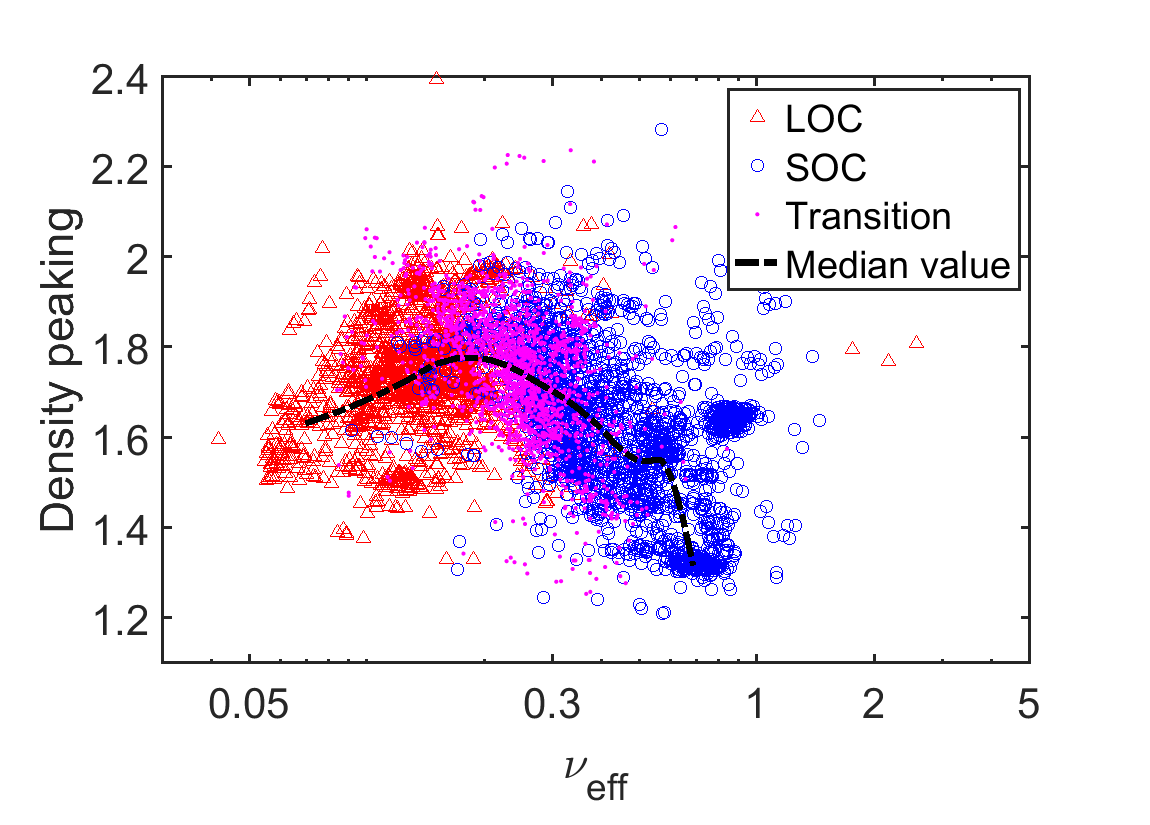
\includegraphics[scale=0.55]{fig_peak_nu_OH_med.eps}
\par\end{centering}
\caption{Plot of the density peaking factor with respect to effective collisionality for Ohmic plasmas with $3 < q_{\psi} <6$.}
\label{fig:peak_nu_OH}
\end{figure}
%%%%%%%%%%%%%%%%%%%%


%This database observed trends of the density peaking with hundreds of Ohmic shots confirms the results of a previous detailed analysis of an Ohmic discharge with an $I_p$ scan (Tore Supra \#48102), supported by GENE gyrokinetic simulations. Linear simulations showed that the TEM instability was destabilized at high $I_p$ (LOC) and stabilized at low $I_p$ (SOC) \cite{Arnichand_2014_NF,Hacquin_2016_PoP,Citrin_2017_PPCF}. Specifically, the increasing trends of the density pealing at high collisionality have extended the previous results to a much wider plasma conditions. Moreover, the decreasing trends of the density pealing at low collisionality provide a new insight to the behaviors of the plasma density profiles or further the particle transport properties. The latter trends night be instructive to the performance enhancement of ITER, which has been predicted to be operated at low collisionality.


\subsection{Dependence of BB component on collisionality}

Having characterized the trend of density peaking in terms of collisionality, linked with a possible change of dominating instability across the LOC-SOC transition, we now proceed to a study of changes in the BB component resulting from the transition. This is based on the BB contribution ($E_\mathrm{BB}$), the BB width ($W_\mathrm{BB}$) and the BB shape ($\beta_\mathrm{BB}$).


\subsubsection{BB contribution}

Figure \ref{fig:EBB_nu_OH} shows the dependence of $E_\mathrm{BB}$ on $\nu_\mathrm{eff}$ in the LOC, SOC and transition regimes at the HFS ($\rho = -0.4$), the plasma center ($\rho = 0$) and the LFS ($\rho = 0.4$). The HFS and LFS radial positions ($\rho = \pm 0.4$) have been chosen to be neither in the region with large radial changes of $E_\mathrm{BB}$ ($0.2 < |\rho| <0.3$), nor in the saturation region ($\rho > 0.6$) (see figure \ref{fig:ELS_med}). At each $\rho$, the data include all the $q_{\psi}$ ranges shown in figure \ref{fig:ELS_med}. Note that $\nu_\mathrm{eff}$ was estimated from the local values of $n_\mathrm{e}$ and $T_\mathrm{e}$. For $Z_\mathrm{eff}$, again the estimate from a tangential line-of-sight was used to calculate $\nu_\mathrm{eff}$. It is strongly weighted by the plasma core, so even if $Z_\mathrm{eff}$ would increase toward the edge, all data points at the LFS and HFS would merely shift slightly toward higher $\nu_\mathrm{eff}$ (under the assumption that the shape of the $Z_\mathrm{eff}$ profile does not change drastically with increasing $\nu_\mathrm{eff}$).


%%%%%%%%%%%%%%%%%%%%
\begin{figure}[h]
\begin{centering}
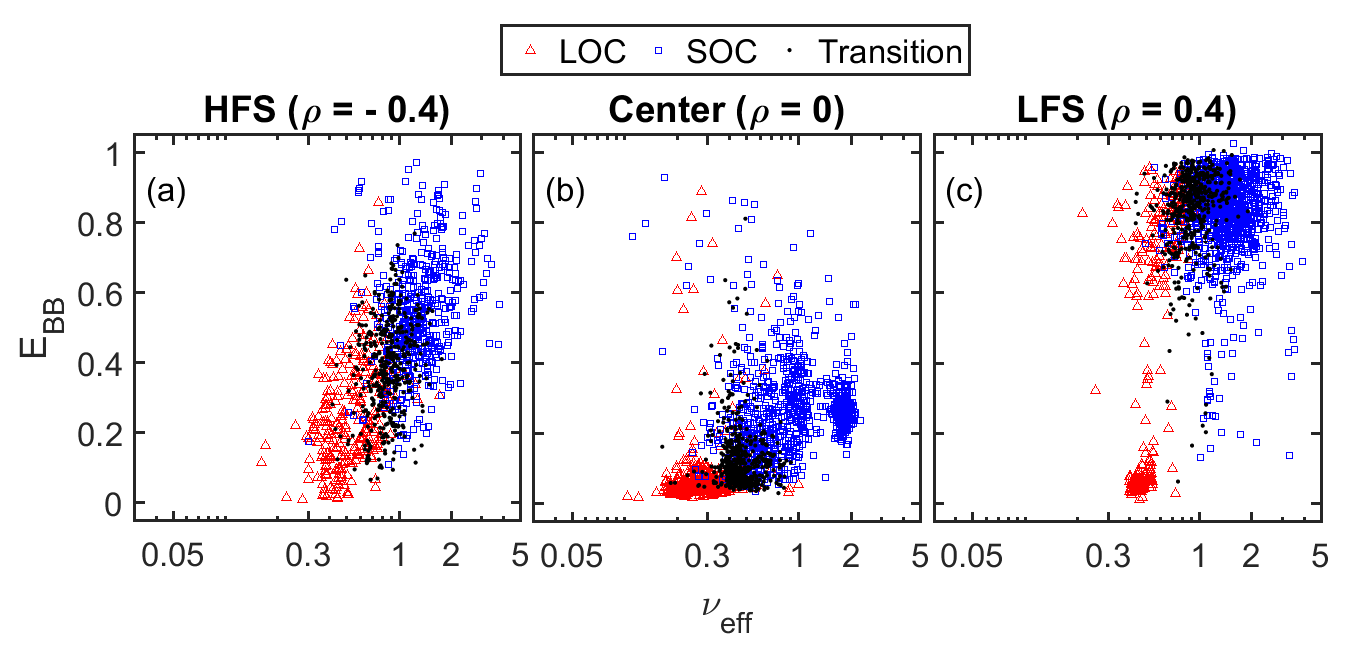
\includegraphics[scale=0.7]{fig_EBB_nu_OH.eps}
\par\end{centering}
\caption{Broadband contribution ($E_\mathrm{BB}$) vs. effective collisionality ($\nu_\mathrm{eff}$) in the LOC, SOC and transition regimes at (a) the HFS ($\rho = -0.4$), (b) the plasma center inside the basin ($\rho = 0$) and (c) the LFS ($\rho = 0.4$). Note the logarithmic scale for $\nu_\mathrm{eff}$.}
\label{fig:EBB_nu_OH}
\end{figure}
%%%%%%%%%%%%%%%%%%%%

Despite the significant scatter of $E_\mathrm{BB}$ in the plots, the following observations can be made. Inside the central $E_\mathrm{BB}$ basin (figure \ref{fig:EBB_nu_OH} (b)), in the LOC regime, $E_\mathrm{BB}$ remains low ($\sim 0.1$) for $\nu_\mathrm{eff}$ ranging from below 0.1 to around 0.3. Above $\nu_\mathrm{eff} = 0.3$, $E_\mathrm{BB}$ generally increases rapidly as the plasma transits from the LOC to the SOC regime. Outside the basin (figure \ref{fig:EBB_nu_OH} (a) and (c)), $\nu_\mathrm{eff}$ (calculated from local $n_\mathrm{e}$ and $T_\mathrm{e}$) is generally higher than in the center, due to the stronger dependence of $\nu_\mathrm{eff}$ on $T_\mathrm{e}$ than on $n_\mathrm{e}$ (from \eqref{eq:Zeff}: $\nu_\mathrm{eff} \propto T_\mathrm{e}^{-2}$ and $\nu_\mathrm{eff}\propto n_\mathrm{e}$), while generally a $T_\mathrm{e}$ profile is steeper than an $n_\mathrm{e}$ profile. At the HFS (figure \ref{fig:EBB_nu_OH} (a)), $E_\mathrm{BB}$ increases almost linearly when $\nu_\mathrm{eff}$ changes from 0.3 to 3 on a logarithmic scale. At the LFS (figure \ref{fig:EBB_nu_OH} (c)), $E_\mathrm{BB}$ also increases with $\nu_\mathrm{eff}$, but it quickly reaches values close to saturation when $\nu_\mathrm{eff} > $ 0.5. Note that a cluster of spectra accumulates at $\nu_\mathrm{eff} \sim 0.5$ when $E_\mathrm{BB} < 0.2$. This remarkable cluster corresponds to the cluster in figure \ref{fig:ELS} (LOC case with $4 < q_{\psi} < 5$). A preliminary investigation has pointed out that the spectra making up this cluster correspond to a number of contiguous Tore Supra discharges (\#40481 -- \#40490). These measurements come from the same acquisition channel and have the same probing frequency (120 GHz), indicating a possible technical problem of this channel for this series of discharges.


Although here the results at only three radial positions are presented, similar trends have been observed at other radial positions, except close to the plasma edge, where saturation occurs. The saturation could be due to an increase of the fluctuation level close to the plasma edge in combination with stronger nonlinear effects. In summary, an increasing trend of $E_\mathrm{BB}$ with $\nu_\mathrm{eff}$ is consistently observed throughout the entire plasma cross-section. Inside the $E_\mathrm{BB}$ basin, at low $\nu_\mathrm{eff}$ the increase is relatively weak, becoming steeper above $\nu_\mathrm{eff} = 0.3$.


%%%%%%%%%%%%%%%%%%%%
\begin{figure}[h]
\begin{centering}
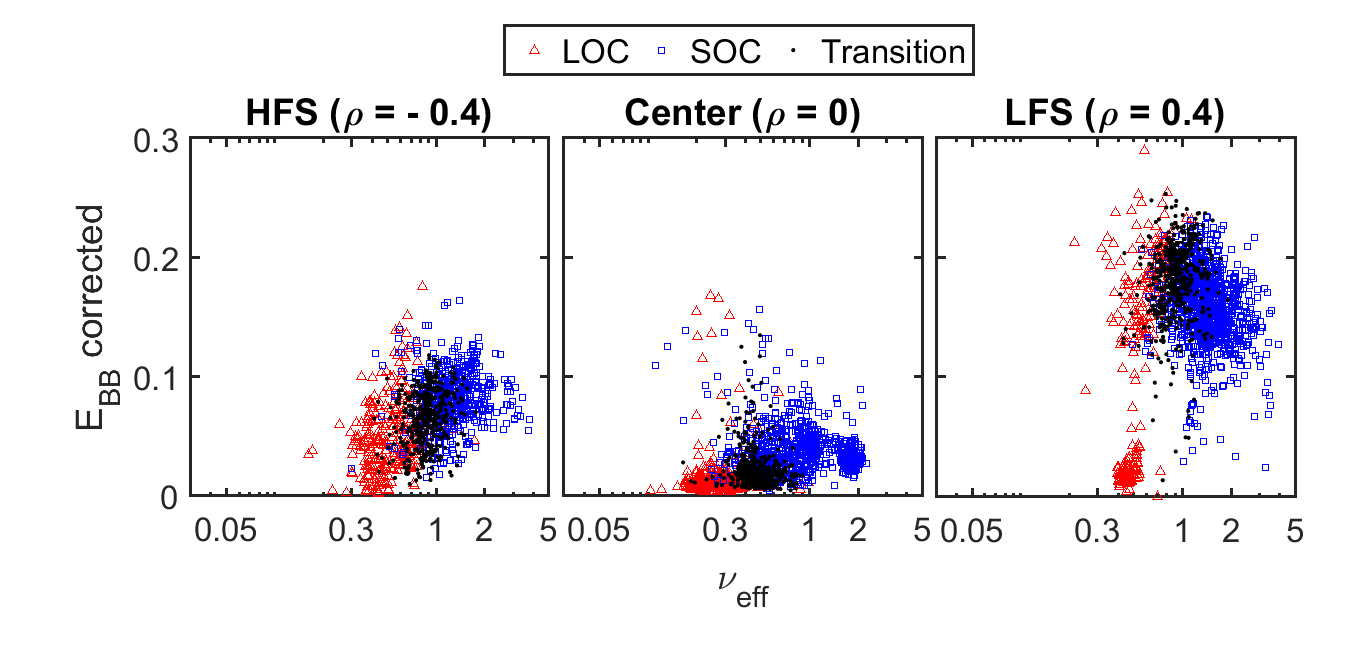
\includegraphics[scale=0.72]{fig_EBBc_nu_OH.eps}
\par\end{centering}
\caption{Corrected $E_\mathrm{BB}$ vs. $\nu_\mathrm{eff}$ in the LOC, SOC and transition regimes at (a) the HFS ($\rho = -0.4$), (b) the plasma center inside the basin ($\rho = 0$) and (c) the LFS ($\rho = 0.4$). Note the logarithmic scale for $\nu_\mathrm{eff}$.}
\label{fig:EBBc_nu_OH}
\end{figure}
%%%%%%%%%%%%%%%%%%%%


Furthermore, after considering the scale length of the refraction index ($L_{\epsilon}$) and the frequency of the probing wave ($\lambda_0$), the dependence of the corrected $E_\mathrm{BB}$ on $\nu_\mathrm{eff}$ at different positions is shown in figure \ref{fig:EBBc_nu_OH}. Generally, similar trends of $E_\mathrm{BB}$ are recovered, as is clear from figure \ref{fig:EBB_nu_OH}. The only difference comes from the high $\nu_\mathrm{eff}$ at the LFS (figure \ref{fig:EBBc_nu_OH} (c)), where a decrease of the corrected $E_\mathrm{BB}$ with $\nu_\mathrm{eff}$ is observed.





\subsubsection{BB width and shape}

In addition to studying the broadband contribution through $E_\mathrm{BB}$, we have also investigated in a similar way the width ($W_\mathrm{BB}$) and shape ($\beta_\mathrm{BB}$) of the BB component. As mentioned in section \ref{sec:parameters_turbulence_database}, $W_\mathrm{BB}$ is obtained from the Taylor model due to its more stable behavior, while $\beta_\mathrm{BB}$ from the generalized Gaussian provides the most direct interpretation of the spectral shape. Specifically, $\beta_\mathrm{BB} = 2$ and $\beta_\mathrm{BB} = 1$ correspond to the standard Gaussian and double exponential shape, respectively, while the Lorentzian shape occurs for $\beta_\mathrm{BB}\lesssim 1$.

Figure \ref{fig:WBB_nu_OH} (a--c) shows the evolution of the BB width $W_\mathrm{BB}$ with $\nu_\mathrm{eff}$ at different $\rho$. Inside the central basin (figure \ref{fig:WBB_nu_OH} (b)), unlike $E_\mathrm{BB}$, $W_\mathrm{BB}$ does not change much with $\nu_\mathrm{eff}$ and remains around 50 kHz. At the HFS (figure \ref{fig:WBB_nu_OH} (a)), $W_\mathrm{BB}$ increases and decreases with $\nu_\mathrm{eff}$ in LOC and SOC regime, respectively, resulting in a maximum $W_\mathrm{BB}$ value at the transition. However, at the LFS (figure \ref{fig:WBB_nu_OH} (c)) where $E_\mathrm{BB}$ is close to saturation (figure \ref{fig:EBB_nu_OH} (c)), the pattern is more complicated. One may distinguish two main clusters: one with $W_\mathrm{BB}>$ 100 kHz, roughly increasing with $\nu_\mathrm{eff}$, and the other with $W_\mathrm{BB}$ remaining approximately at $\sim 50$ kHz, even at high $\nu_\mathrm{eff}$. Another interesting observation is that $W_\mathrm{BB}$ tends to be scattered the most in the transition regions, where different types of instabilities might co-exist.

Figure \ref{fig:WBB_nu_OH} (d--f) shows the evolution of the BB shape $\beta_\mathrm{BB}$ with $\nu_\mathrm{eff}$ at different $\rho$. No clear trends can be discerned, but a few observations can be made. First, in the plasma center, the dispersion of $\beta_\mathrm{BB}$ is clearly larger in the LOC regime than in the SOC regime. Second, at high $\nu_\mathrm{eff}$, the $\beta_\mathrm{BB}$ values tend to cluster around 1, corresponding to a double exponential shape.
%%%%%%%%%%%%%%%%%%%%
\begin{figure}[h]
\begin{centering}
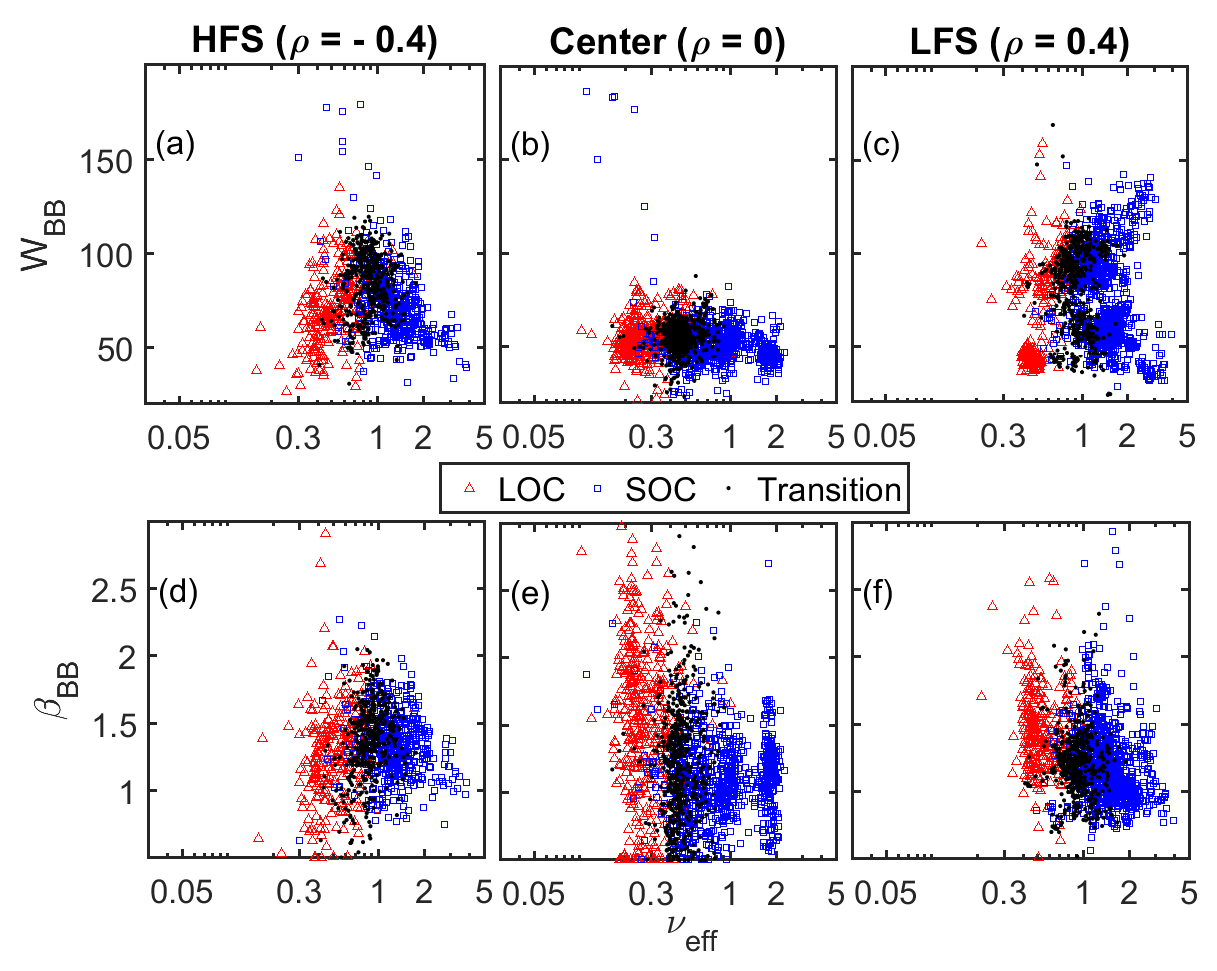
\includegraphics[scale=0.75]{fig_WBB_betaBB_nu_OH.eps}
\par\end{centering}
\caption{Similar to figure \ref{fig:EBB_nu_OH} for the evolution of the broadband width $W_\mathrm{BB}$ and shape $\beta_\mathrm{BB}$.}
\label{fig:WBB_nu_OH}
\end{figure}
%%%%%%%%%%%%%%%%%%%%


\subsection{Interpretation of spectrum dependencies on confinement regime}

We propose a possible interpretation of the observed trends of the BB component in terms of $\nu_\mathrm{eff}$ by a change of the dominant instability from TEM to ITG, when crossing from the LOC to the SOC regime. This interpretation is suggested by the dependence of density peaking on collisionality in figure \ref{fig:peak_nu_OH}. Furthermore, it is lent by an earlier, dedicated study of the effect of the dominant instability on the density fluctuation spectra by gyrokinetic simulations in the Ohmic Tore Supra discharge \#48102 \cite{Arnichand_2016_PPCF,Citrin_2017_PPCF}. The simulations were performed at $\rho = 0.37$, which is close to the position in the database study ($\rho = 0.4$) at the LFS. Figure \ref{fig:simu_spec} shows that, in the LOC regime when TEM dominates, the BB component is separated from a narrow LF component, whereas in the SOC regime when ITG dominates, a much wider BB component exists and the LF component merges into the BB component.


%%%%%%%%%%%%%%%%%%%%
\begin{figure}[h]
\begin{centering}
\includegraphics[scale=0.8]{fig_simu_spec_TEM_ITG_gray.eps}
\par\end{centering}
\caption{Density fluctuation spectra by gyrokinetic simulations in Tore Supra discharge \#48102 at $\rho = $ 0.37 for (a) the LOC and (b) the SOC regime. Reprinted from Refs \cite{Arnichand_2016_PPCF}, copyright owned by IOP Publishing.}
\label{fig:simu_spec}
\end{figure}
%%%%%%%%%%%%%%%%%%%%


To support this interpretation, we have studied the radial profiles of the LF width ($W_\mathrm{LF}$) in the LOC and SOC regimes, as shown in figure \ref{fig:WLF_r_OH}. It is clear that $W_\mathrm{LF}$ in the SOC regime is systematically higher than in the LOC regime at all radial positions. Specifically, at the center inside the $q = 1$ surface, the LF width in the SOC regime ($\sim$ 8 kHz) is approximately two times the width in the LOC regime ($\sim$ 4 kHz). However, the estimate of $W_\mathrm{LF}$ from our parametrization technique might be less reliable when the BB contribution is high. From figure \ref{fig:ELS_med}, outside the central basin, i.e. outside the $q = 1$ surface, $E_\mathrm{BB}$ may reach a value of 0.5 (HFS) or close to 1 (LFS). Accordingly, when $E_\mathrm{BB}$ is close to 1, most of the energy is in the BB component and the LF component disappears or merges with the BB component, rendering the fit of the LF component, and thus $W_\mathrm{LF}$, unstable. Therefore, we focus only on the HFS and the core region, where $E_\mathrm{BB}$ is not close to 1 (saturation) and thus $W_\mathrm{LF}$ is more reliable.


%%%%%%%%%%%%%%%%%%%%
\begin{figure}[h]
\begin{centering}
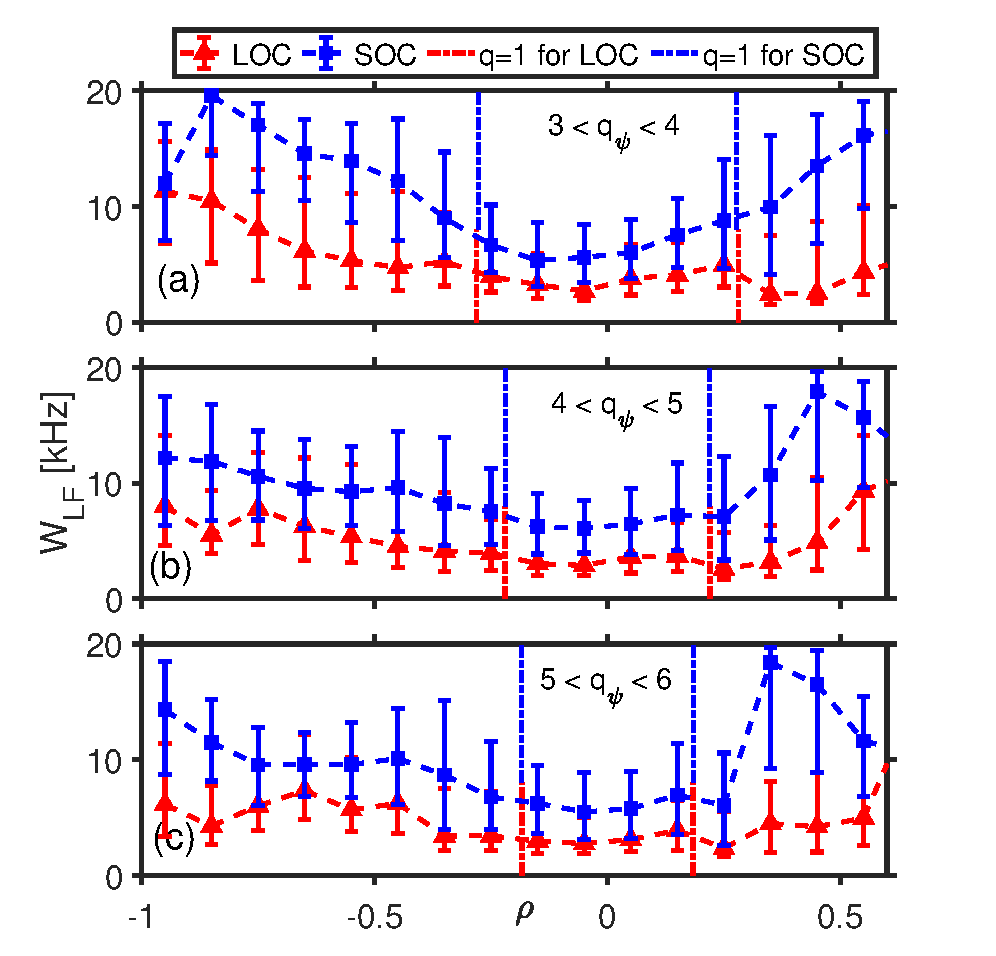
\includegraphics[scale=0.67]{fig_WLF_LOCSOC.eps}
\par\end{centering}
\caption{Median radial profiles of the LF width $W_\mathrm{LF}$ at different ranges of the edge safety factor ($q_{\psi}$) in the LOC and SOC regimes.}
\label{fig:WLF_r_OH}
\end{figure}
%%%%%%%%%%%%%%%%%%%%


Figures \ref{fig:WLF_nu_OH} (a) and (b) show the dependence of the LF width ($W_\mathrm{LF}$) on $\nu_\mathrm{eff}$ at the HFS ($\rho = -0.4$) and at the center ($\rho = 0$), respectively. At the center (figure \ref{fig:WLF_nu_OH} (b)), $W_\mathrm{LF}$ increases slowly with $\nu_\mathrm{eff}$ in both LOC and SOC regime, with the weakest slope in SOC. As far as the LF magnitude is concerned, most of $W_\mathrm{LF}$ in the LOC regime is around or below 5 kHz, whereas $W_\mathrm{LF}$ in the SOC regime could be near 10 kHz, which is consistent with the systematic observations near the core region in figure \ref{fig:WLF_r_OH}. However, note that the trends are difficult to extract due to the strong dispersion of the data points, especially during the transition regime. This strong data dispersion is also observed at the HFS (figure \ref{fig:WLF_nu_OH} (a)), where a much faster increase of $W_\mathrm{LF}$ with $\nu_\mathrm{eff}$ seems to exist.

The generally observed increasing trends of the LF width, as the confinement regime changes from LOC to SOC in figures \ref{fig:WLF_r_OH} and \ref{fig:WLF_nu_OH}, are consistent with the GENE simulations in figure \ref{fig:simu_spec}. This supports the interpretation that the observed changes of the BB component in the frequency spectra can be induced by a change of dominating instability from TEM to ITG.


%%%%%%%%%%%%%%%%%%%%
\begin{figure}[h]
\begin{centering}
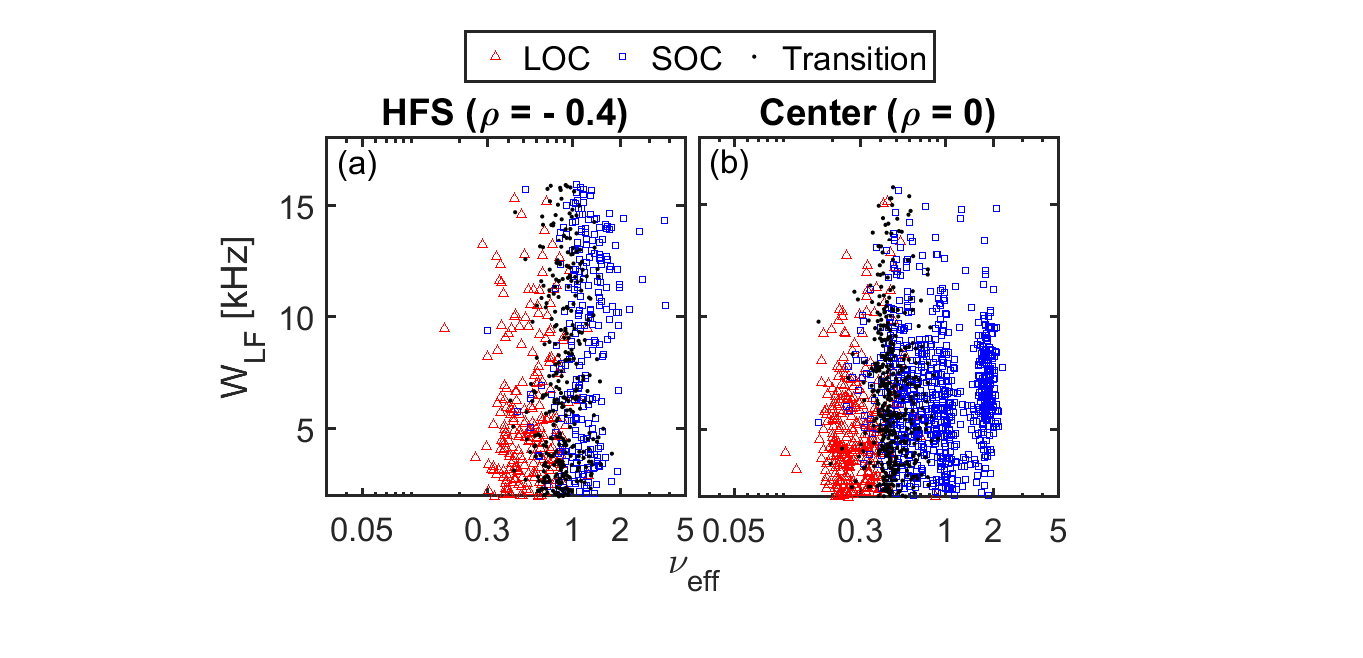
\includegraphics[scale=0.8]{fig_WLF_nu_r0_HFS_OH.eps}
\par\end{centering}
\caption{LF width ($W_\mathrm{LF}$) vs. effective collisionality ($\nu_\mathrm{eff}$) in the LOC, SOC and transition regimes at (a) the HFS ($\rho = -0.4$), (b) the plasma center inside the basin ($\rho = 0$).}
\label{fig:WLF_nu_OH}
\end{figure}
%%%%%%%%%%%%%%%%%%%%


\section{Frequency spectrum in plasmas with auxiliary power} \label{sec:spec_Lmode}


After studying the change of spectral characteristics with collisions in Ohmic plasmas, the nest step is to study the spectral characteristics with additional heating power.


\subsection{Dependence of BB component on collisionality}

To better understand the different levels of $E_\mathrm{BB}$ in L-mode with ICRH or LH heating, the dependence of $E_\mathrm{BB}$ on effective collisionality has been analyzed as well. Calculations of $\nu_\mathrm{eff}$ are more complicated in L-mode, because measurements of $Z_\mathrm{eff}$ from bremsstrahlung spectroscopy can be less reliable in Tore Supra LH discharges, reaching very large values ($\gtrsim$ 6). It was previously reported that hot spots on the inner wall, supra-thermal electrons and influence of reflections may cause overestimation of $Z_\mathrm{eff}$ in Tore Supra LH plasmas. \cite{Schunke_2005_RSI} Therefore, a robust multi-machine scaling law \cite{Matthews_1997_JNM} has been used to obtain $Z_\mathrm{eff}$ in LH plasmas:%
%%%%%%%%%%%%%%%%%%%%
\begin{equation}\label{eq:Zeff}
  Z_\mathrm{eff} = 1 + 7\frac{P_\mathrm{rad}}{S n_l^2},
\end{equation}
%%%%%%%%%%%%%%%%%%%%
\noindent Here, $P_\mathrm{rad}$ is the total radiated power in MW, $S=4\pi^2Ra$ the plasma surface area in m$^2$ and $n_\mathrm{l}$ the line-averaged density in 10$^{-20}$ m$^{-3}$, all available in the database. In ICRH plasmas the problem is less severe, but the scaling law has also been used in this case to maintain consistency with the LH case.


\subsubsection{BB contribution}

Figure \ref{fig:EBB_nu_Lmode} shows a plot of $E_\mathrm{BB}$ on $\nu_\mathrm{eff}$ at different $\rho$. The value of $\nu_\mathrm{eff}$ is systematically lower here than in Ohmic plasmas, due to the higher $T_\mathrm{e}$ with additional heating. Inside the central basin (figure \ref{fig:EBB_nu_Lmode} (b)), the LH plasmas dominate in the low $\nu_\mathrm{eff}$ ranges. In this region, most of $E_\mathrm{BB}$ in LH plasmas remains at a low level ($\sim 0.2$) for $\nu_\mathrm{eff} < $ 0.3, when Ohmic plasmas are in LOC regime (figure \ref{fig:EBB_nu_OH} (b)). The ICRH plasmas dominate in the higher $\nu_\mathrm{eff}$ ranges and most of $E_\mathrm{BB}$ in ICRH is above 0.5 with strong dispersion. Regardless of the heating method, the general increasing trend of $E_\mathrm{BB}$ with $\nu_\mathrm{eff}$ observed in Ohmic plasmas is recovered, not only inside but also outside the basin. Furthermore, at the LFS (figure \ref{fig:EBB_nu_Lmode} (c)), $E_\mathrm{BB}$ in LH, and probably also ICRH, is close to saturation at large $\nu_\mathrm{eff}$, while at the HFS (figure \ref{fig:EBB_nu_Lmode} (a)) saturation of $E_\mathrm{BB}$ only occurs with ICRH. It should be noted that relatively few plasmas are available in the database with ICRH at the LFS (figure \ref{fig:EBB_nu_Lmode} (c)), somewhat degrading the reliability of the results under these conditions. This is due to a lack of valid spectra caused by a strong Doppler effect, which often affects the spectra towards the LFS.


%%%%%%%%%%%%%%%%%%%%
\begin{figure}[h]
\begin{centering}
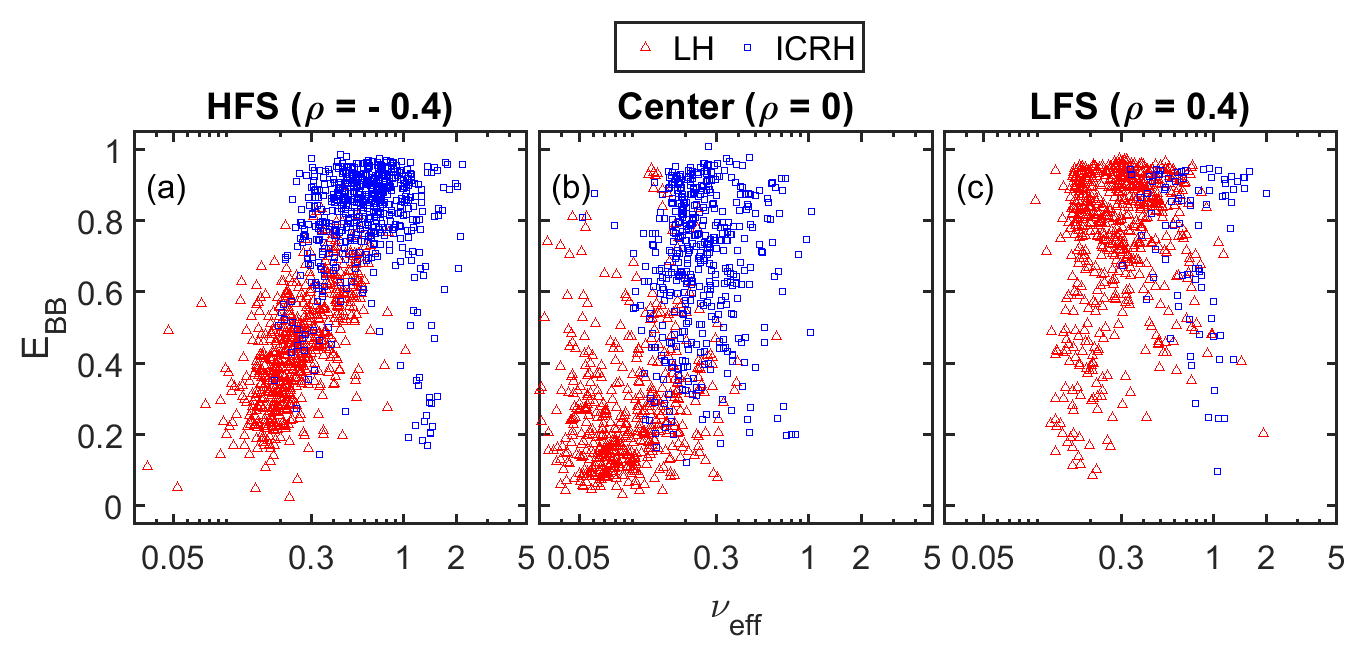
\includegraphics[scale=0.7]{fig_EBB_nu_Lmode.eps}
\par\end{centering}
\caption{Broadband contribution ($E_\mathrm{BB}$) vs. effective collisionality ($\nu_\mathrm{eff}$) in L-mode with pure ICRH or LH at different positions. Only plasmas with moderate heating power (1 MW $<P_\mathrm{heat}< 3$ MW) are shown.}
\label{fig:EBB_nu_Lmode}
\end{figure}
%%%%%%%%%%%%%%%%%%%%


Following the discussion in the Ohmic cases, the trend of the corrected $E_\mathrm{BB}$ with $\nu_\mathrm{eff}$ has also been studied, shown in figure \ref{fig:EBBc_nu_Lmode}. Similar trends as in figure \ref{fig:EBB_nu_Lmode} are observed at different positions. However, the systematically higher magnitude of the BB contribution at the LFS, compared to the HFS, can be deduced from the corrected $E_\mathrm{BB}$ but not from $E_\mathrm{BB}$. Most notably, the possible decreasing trend at high $\nu_\mathrm{eff}$ at the LFS (figure \ref{fig:EBBc_nu_Lmode} (c)) is more clear compared with figure \ref{fig:EBBc_nu_OH} (c), although this needs to be investigated in more detail.


%%%%%%%%%%%%%%%%%%%%
\begin{figure}[h]
\begin{centering}
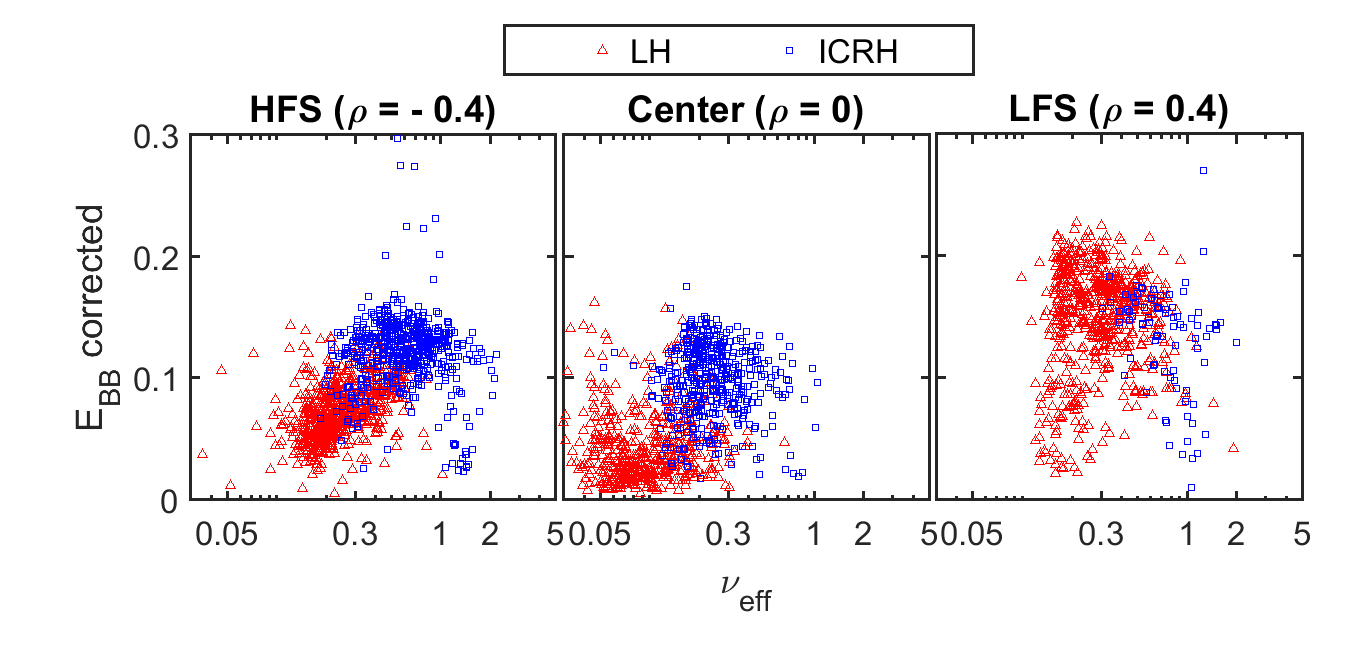
\includegraphics[scale=0.72]{fig_EBBc_nu_Lmode.eps}
\par\end{centering}
\caption{Corrected $E_\mathrm{BB}$ vs. effective collisionality ($\nu_\mathrm{eff}$) in L-mode with pure ICRH or LH at different positions. Only plasmas with moderate heating power (1.5 MW $<P_\mathrm{heat}< 2.5$ MW) are shown.}
\label{fig:EBBc_nu_Lmode}
\end{figure}
%%%%%%%%%%%%%%%%%%%%


\subsubsection{BB width and shape}

We next study the dependence of the broadband width $W_\mathrm{BB}$ and shape $\beta_\mathrm{BB}$ on collisionality with ICRH and LH. Figure \ref{fig:WBB_nu_Lmode} (a--c) shows the dependence of $W_\mathrm{BB}$ on $\nu_\mathrm{eff}$ at different $\rho$. In contrast to the Ohmic case, a relatively clear increasing trend of $W_\mathrm{BB}$ can be observed with $\nu_\mathrm{eff}$ in LH plasmas. For the ICRH plasmas, operating at higher $\nu_\mathrm{eff}$, no clear trends of $W_\mathrm{BB}$ with $\nu_\mathrm{eff}$ can be observed at the HFS. Moreover, in absolute terms, the scatter of $W_\mathrm{BB}$ appears to be lower with LH than ICRH. Another noticeable feature of $W_\mathrm{BB}$ lies in a systematic increase from inside the basin towards the HFS or LFS. This feature is the most pronounced with ICRH, where $W_\mathrm{BB}$ increases from around 100 kHz to 150 kHz and above.

Likewise, figure \ref{fig:WBB_nu_Lmode} (d--f) shows the evolution of $\beta_\mathrm{BB}$ from the generalized Gaussian model with $\nu_\mathrm{eff}$, with ICRH or LH at different $\rho$. Similar to the Ohmic case, in the plasma center at lower collisionalities, corresponding to LH heating, the dispersion of $\beta_\mathrm{BB}$ is larger than with ICRH heating. Indeed, at higher $\nu_\mathrm{eff}$, the $\beta_\mathrm{BB}$ values cluster around $\sim 1$ (double exponential). In addition, like the width, the shape parameter in ICRH plasmas tends to be higher outside the basin than inside.


%%%%%%%%%%%%%%%%%%%%
\begin{figure}[h]
\begin{centering}
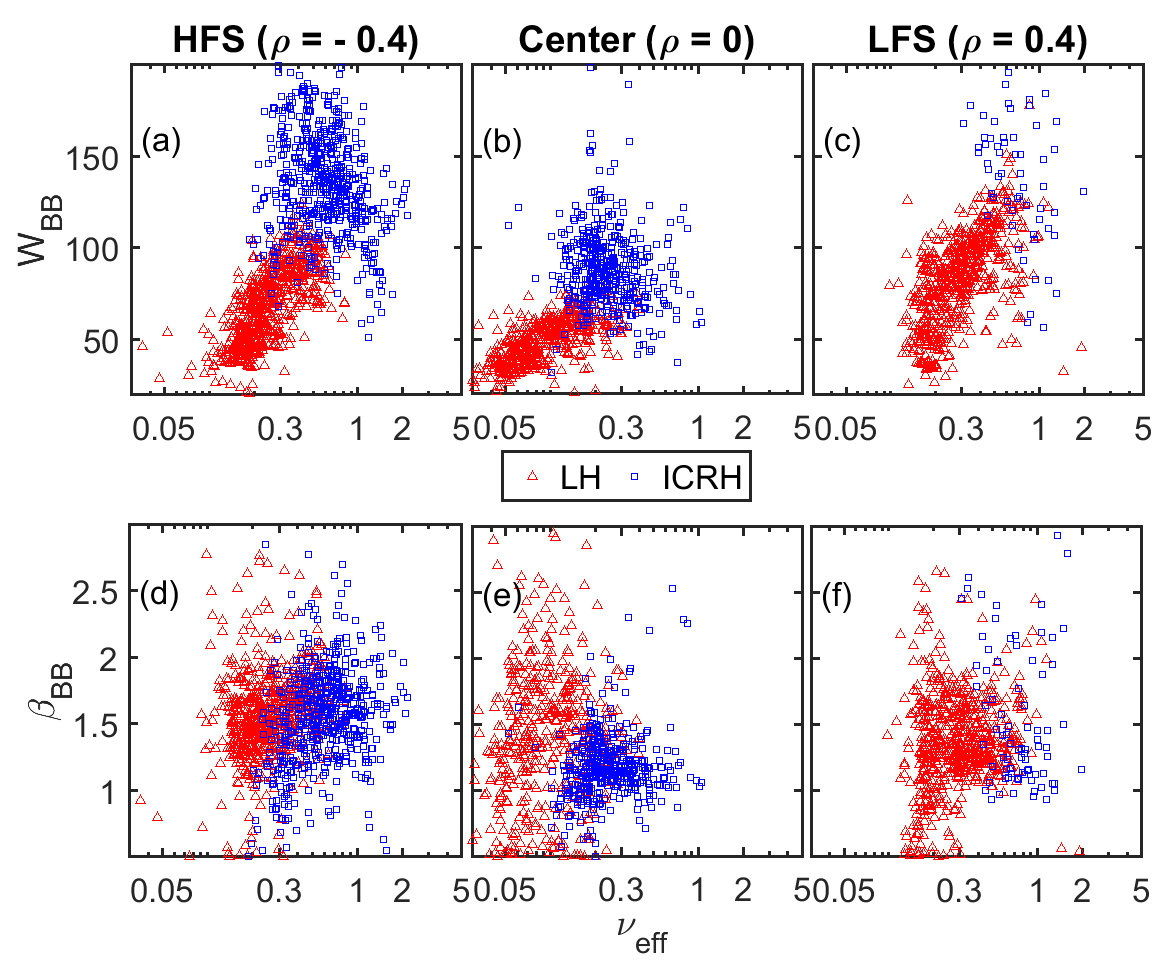
\includegraphics[scale=0.7]{fig_WBB_betaBB_nu_Lmode.eps}
\par\end{centering}
\caption{Same as figure \ref{fig:EBB_nu_Lmode} for the trend of the broadband width $W_\mathrm{BB}$ (a--c) and shape $\beta_\mathrm{BB}$ (d--f).}
\label{fig:WBB_nu_Lmode}
\end{figure}
%%%%%%%%%%%%%%%%%%%%


%%%%%%%%%%%%%%%%%%%%
\begin{figure}[!h]
\begin{centering}
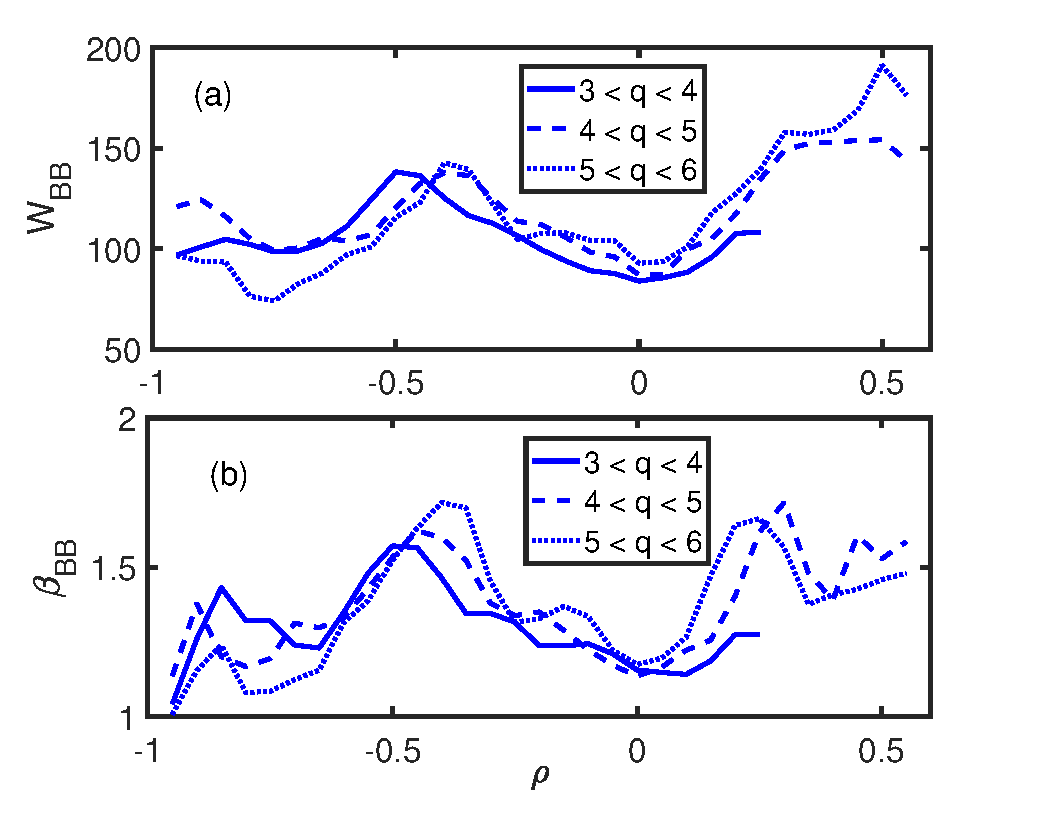
\includegraphics[scale=0.57]{fig_WBB_betaBB_prof.eps}
\par\end{centering}
\caption{Radial profiles of (a) BB width ($W_\mathrm{BB}$) and (b) shape ($\beta_\mathrm{BB}$) with ICRH. Here, median values are plotted based on small radial intervals ($\delta\rho=\pm0.05$), leaving out intervals with insufficient points.}
\label{fig:fig_WBB_betaBB_prof}
\end{figure}
%%%%%%%%%%%%%%%%%%%%


To further investigate the observed radial trends of $W_\mathrm{BB}$ and $\beta_\mathrm{BB}$ in L-mode, especially the systematic change with ICRH when inside or outside the basin, the radial profiles of $W_\mathrm{BB}$ and $\beta_\mathrm{BB}$ in ICRH plasmas at different $q_{\psi}$ are shown in figure \ref{fig:fig_WBB_betaBB_prof} (a) and (b), respectively. These are median profiles calculated from all relevant plasmas in the database. In figure \ref{fig:fig_WBB_betaBB_prof} (a), $W_\mathrm{BB}$ exhibits a local minimum inside the central basin. At the HFS around $\rho\sim -0.3$ to $-0.6$, $W_\mathrm{BB}$ shows a bump structure, which is shifted towards the plasma center with increasing $q_{\psi}$ ranges, whereas saturation occurs at the LFS. This corresponds to the observations in figure \ref{fig:WBB_nu_Lmode} (d--f). Since $W_\mathrm{BB}$ is related to the plasma rotation, the bump structure could be linked to a change of rotation velocity shear at the HFS, although this needs further investigation. A similar bump structure and its relation to $q_{\psi}$ ranges occurs for the radial profiles of $\beta_\mathrm{BB}$, as shown in figure \ref{fig:fig_WBB_betaBB_prof} (b).


%\subsection{Other observations with increasing $\nu_\mathrm{eff}$}


\subsection{Trends for the LF component}

We have also investigated the radial profiles of the LF width ($W_\mathrm{LF}$) with ICRH and LH at different ranges of $q_{\psi}$, as shown in figure \ref{fig:WLF_r_Lmode}. It is clear that $W_\mathrm{LF}$ with ICRH is systematically higher than with LH at almost all radial positions. Specifically, $W_\mathrm{LF}$ with LH is usually around 5 kHz, whereas $W_\mathrm{LF}$ with ICRH is close to 20 kHz (saturation) for most of the situations. Note that the saturation of $W_\mathrm{LF}$ is an artifact of the fitting procedure, reaching the upper constraint of 20 kHz on $W_\mathrm{LF}$. This constraint cannot be relaxed, however, to allow distinguishing between the BB and LF components.


%%%%%%%%%%%%%%%%%%%%
\begin{figure}[h]
\begin{centering}
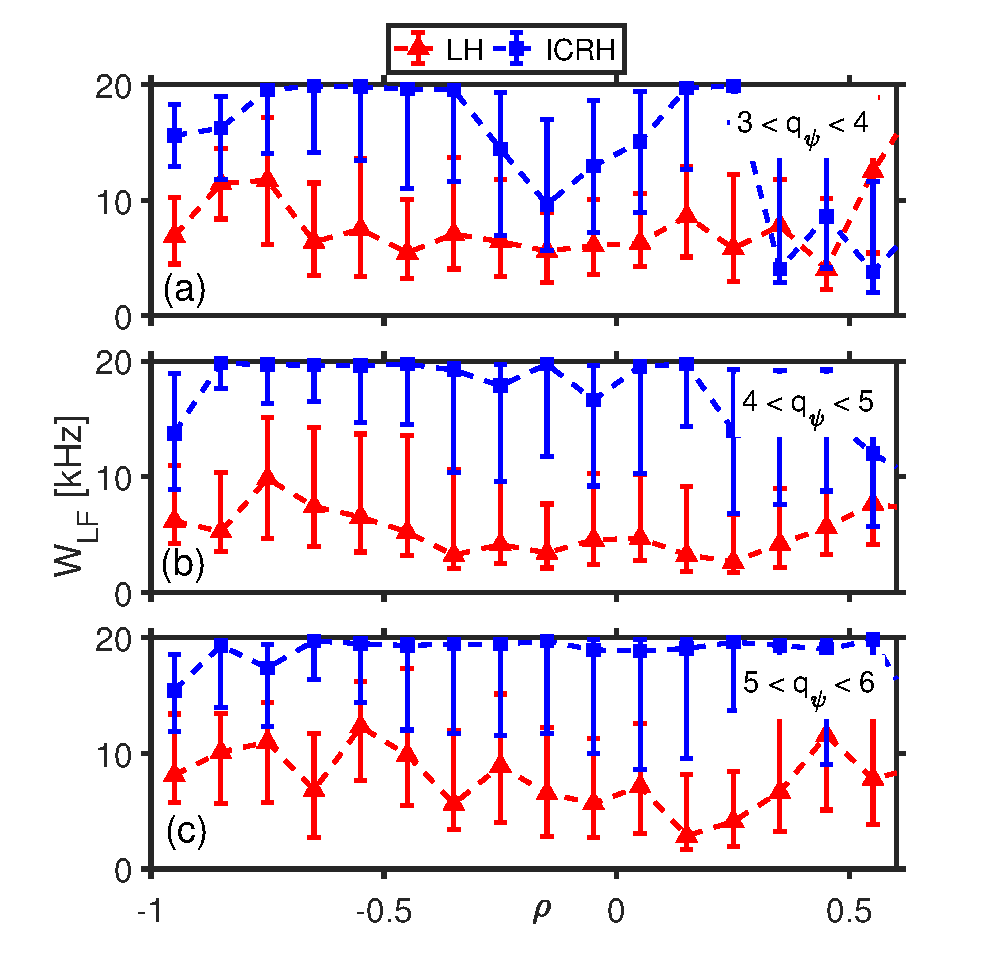
\includegraphics[scale=0.6]{fig_WLF_ICRH_LH.eps}
\par\end{centering}
\caption{Median radial profiles of the LF width ($W_\mathrm{LF}$) at different range of the edge safety factor ($q_{\psi}$) with ICRH and LH.}
\label{fig:WLF_r_Lmode}
\end{figure}
%%%%%%%%%%%%%%%%%%%%



However, as mentioned before, when $B_\mathrm{LF}$ is close to 1 or when $W_\mathrm{LF}$ is close to 20 kHz, the LF component may disappear or merge with the BB component. This degrades the reliability of the observed $W_\mathrm{LF}$ and therefore these circumstances should be avoided. So, when studying the dependence of $W_\mathrm{LF}$ on $\nu_\mathrm{eff}$, these less reliable results are removed by setting $W_\mathrm{LF} < 0.6$ and $W_\mathrm{LF} < 16 $ kHz. Moreover, we have only focused on the HFS and the core region to avoid the strong saturation occurring at the LFS, as shown in figure \ref{fig:WLF_nu_Lmode}. At the HFS (figure \ref{fig:WLF_nu_Lmode} (a)), an increasing trend can be observed, although strong scattering of the data points at fixed $\nu_\mathrm{eff}$ occurs. The data is even more scattered in the center (figure \ref{fig:WLF_nu_Lmode} (a)), possibly with a very weak increasing trend of $W_\mathrm{LF}$ with $\nu_\mathrm{eff}$. However, some low $W_\mathrm{LF}$ data exist at high $\nu_\mathrm{eff}$ in ICRH plasmas, which clearly deviate form the main trend. We have not been able to explain these exceptions, and a deeper shot-to-shot analysis will be required.


%%%%%%%%%%%%%%%%%%%%
\begin{figure}[h]
\begin{centering}
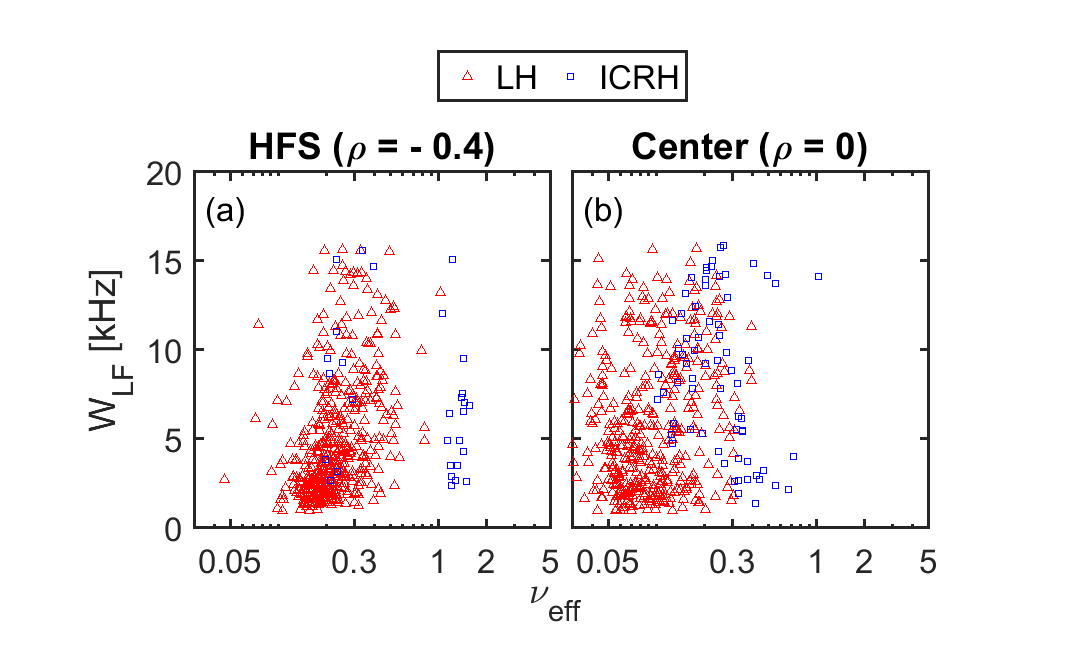
\includegraphics[scale=0.83]{fig_WLF_nu_r0_HFS_Lmode.eps}
\par\end{centering}
\caption{LF width ($W_\mathrm{LF}$) vs. effective collisionality ($\nu_\mathrm{eff}$) in L-mode with pure ICRH or LH at (a) the HFS and (b) the plasma center. Only plasmas with moderate heating power (1.5 MW $< P_\mathrm{heat} <$ 2.5 MW) are shown.}
\label{fig:WLF_nu_Lmode}
\end{figure}
%%%%%%%%%%%%%%%%%%%%


\subsection{Density peaking}

Figure \ref{fig:peak_nu_Lmode} shows the density peaking with respect to the effective collisionality. The density peaking increases slowly with $\nu_\mathrm{eff}$ at lower $\nu_\mathrm{eff}$, corresponding almost exclusively to LH-heated discharges, reaching a maximum value at about $\nu_\mathrm{eff} \sim 0.1$. At higher $\nu_\mathrm{eff}$ ($> 0.1$), the density peaking decreases rapidly with $\nu_\mathrm{eff}$, corresponding mostly to ICRH discharges. The dependence of density peaking on $\nu_\mathrm{eff}$ is thus very similar to the trends observed in the Ohmic case (figure \ref{fig:peak_nu_OH}), expect that the slope at low $\nu_\mathrm{eff}$ is much flatter in LH discharges than in the LOC regime.


%%%%%%%%%%%%%%%%%%%%
\begin{figure}[h]
\begin{centering}
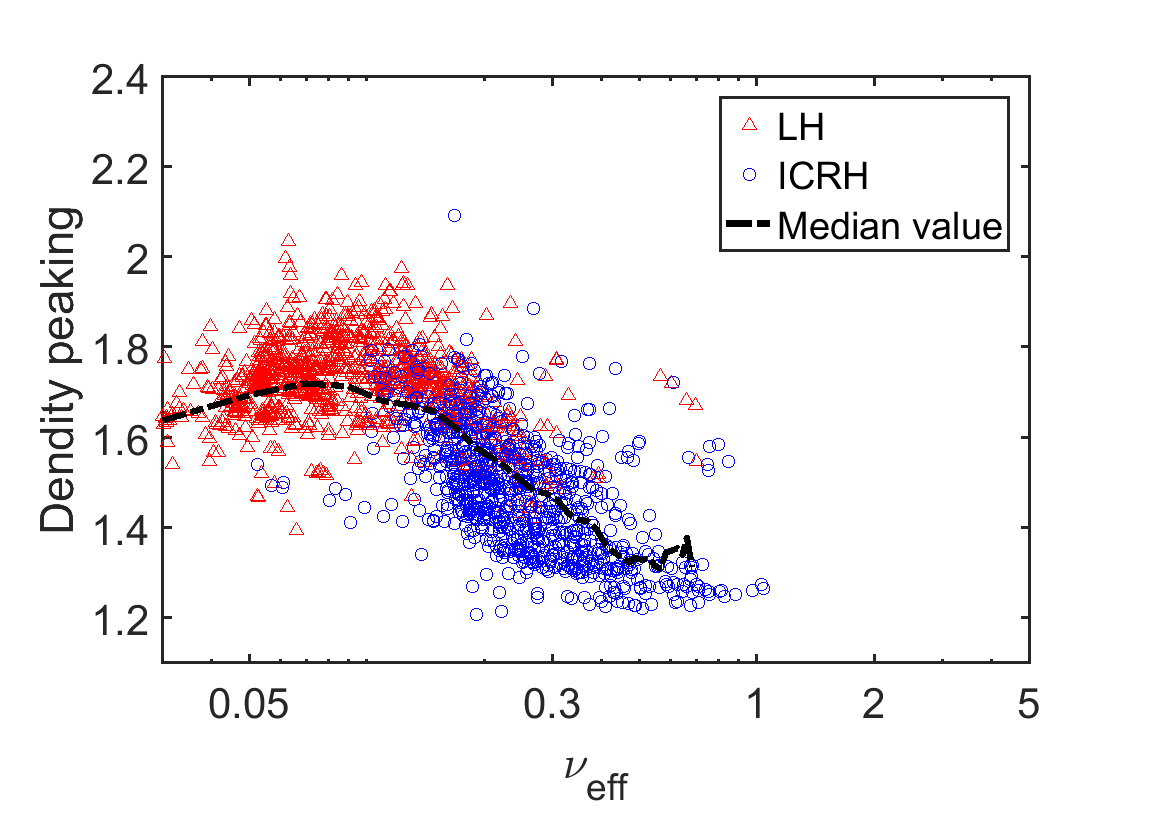
\includegraphics[scale=0.6]{fig_peak_nu_Lmode_med.eps}
\par\end{centering}
\caption{Density peaking factor vs. effective collisionality in L-mode.}
\label{fig:peak_nu_Lmode}
\end{figure}
%%%%%%%%%%%%%%%%%%%%


\subsection{Interpretation}

Given the similarity of the observed trends of $E_\mathrm{BB}$ in terms of $\nu_\mathrm{eff}$ with ICRH or LH, compared to the Ohmic case, one possible explanation is again offered by the stabilization of the TEM instabilities with increasing collisionality. At high collisionality, this would result in discharges where the turbulence would be driven mostly or exclusively by ITG instabilities. The decrease of the density peaking (figure \ref{fig:peak_nu_Lmode}) with $\nu_\mathrm{eff}$ above 0.1 supports this interpretation. Below this threshold, the density peaking increases with $\nu_\mathrm{eff}$, but the slope is weaker than in the Ohmic case (figure \ref{fig:peak_nu_OH}). This might be explained by the current driven by LH waves, reducing the toroidal electric field $E_{\phi}$. Another explanation could be that the turbulence is due to a mix of TEM and ITG instabilities at low $\nu_\mathrm{eff}$ below the threshold. The decrease of the density peaking with $\nu_\mathrm{eff}$ for ITG turbulence would reduce the slope at low $\nu_\mathrm{eff}$ as observed in the LOC regime (figure \ref{fig:peak_nu_OH}).

As for the BB width ($W_\mathrm{BB}$), attempts have been made in the past to connect the width and shape of frequency spectra to the underlying instability, both from the theoretical and experimental viewpoints. \cite{Romanelli_1989_PoF,Mattor_1992_PoF,Watts_1996_PoP}. With the extensive spectrum database, we have identified an increasing trend of the BB width in terms of collisionality in L-mode plasmas with ICRH or LH heating, although no such general trends has been observed in the Ohmic case. The BB width could be linked to both turbulence properties and toroidal intrinsic rotation. In terms of the latter mechanism, one might expect a decrease of $W_\mathrm{BB}$ with increasing collisionality, as the main location where the power is deposited moves outward. The fact that, on the contrary, an increasing trend is observed for the LH plasmas in this database study (figure \ref{fig:WBB_nu_Lmode}), could indicate an unknown link between the BB width and the underlying instabilities. The net effect could be the result of a competition between multiple mechanisms. Therefore, the link between the spectral width of the fluctuation measurements and the turbulence properties or instabilities remains an open question. Note that also the broadband shape could be an important factor in a systematic study, due to its connection with the BB width. Although only weak trends have been observed for the BB shape for both Ohmic and L-mode plasmas (not shown here), other or additional plasma parameters might be used to simultaneously explain the BB width and shape in future work.


\section{Discussion and perspectives} \label{discussion_perspective}

In this chapter, we have studied trends of the BB component with collisionality in both Ohmic and L-mode plasmas with ICRH or LH. We have proposed a possible transition of the dominating instability to explain the observations, supported by earlier gyrokinetic simulations and a study of the density peaking and the LF component.

To put the proposed interpretation on firmer ground, one would need to identify a number of discharges in the database that are sufficiently diagnosed to enable transport analysis with a view to validated profiles of density, temperature, current and impurity concentrations. Then, quasi-linear gyrokinetic simulations with the QuaLiKiz code \cite{Bourdelle_2007_PoP_Qualikiz} or with gyrokinetic codes such as GENE could be performed to compute the growth rates of the different instabilities and deduce the dominant ones. In a next step, ones would perform nonlinear gyrokinetic simulations to obtain density fluctuation maps. Full-wave reflectometry simulations could then be run to obtain frequency fluctuation spectra that could be compared to the experimental measurements.

The trends that have been observed through the present database study, in combination with an efficient spectrum parametrization, must be confirmed through simulations and dedicated experiments, taking into account that some circumstances have changed with the upgrade from Tore Supra to the WEST tokamak. Furthermore, there are many ways in which the present study could be improved. The strong dispersion of the data suggests that dependencies on additional plasma parameters may need to be taken into account to characterize trends of the fluctuation spectra. On the other hand, while the individual parameters used to characterize each spectrum may be interpreted from the physical point of view, each of them only quantifies a certain aspect of the spectrum.  The parametrization method could be augmented with modern techniques from data science, enabling a more integrated quantification of shapes and distributions \cite{Shabbir_2016_RSI}. Combined with advanced regression analysis, this could contribute to systematic studies of the characteristics of micro-instabilities in terms of varying plasma conditions. Equipped with a similarity measure between frequency spectra, classification techniques could help discriminating between turbulent regimes based on the shape of their spectra.
